\begin{figure}[t]
\centering
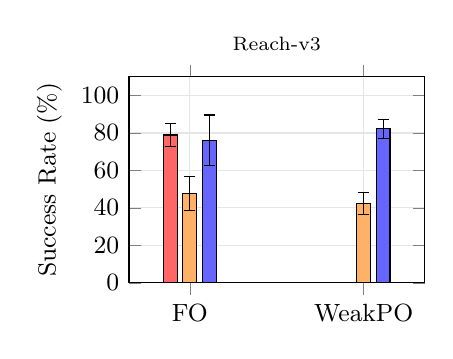
\begin{tikzpicture}
\begin{axis}[
    ybar,
    width=0.44\textwidth,
    height=4.2cm,
    bar width=5pt,
    ymin=0, ymax=110,
    ytick={0,20,40,60,80,100},
    symbolic x coords={FO, WeakPO},
    xtick=data,
    enlarge x limits=0.35,
    grid=major,
    grid style={gray!20},
    ylabel={Success Rate (\%)},
    error bars/y dir=both,
    error bars/y explicit,
    tick label style={font=\small},
    label style={font=\small},
    title={\scriptsize Reach-v3},
]
\addplot[fill=red!60] coordinates {(FO,78.9) +- (0,6.0) (WeakPO,0.0) +- (0,0.0)};
\addplot[fill=orange!60] coordinates {(FO,47.8) +- (0,9.0) (WeakPO,42.2) +- (0,5.9)};
\addplot[fill=blue!60] coordinates {(FO,76.1) +- (0,13.5) (WeakPO,82.2) +- (0,5.0)};
\end{axis}
\end{tikzpicture}
\hfill
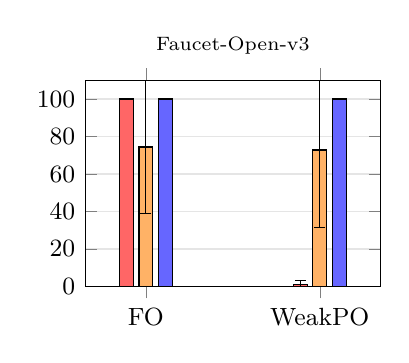
\begin{tikzpicture}
\begin{axis}[
    ybar,
    width=0.44\textwidth,
    height=4.2cm,
    bar width=5pt,
    ymin=0, ymax=110,
    ytick={0,20,40,60,80,100},
    symbolic x coords={FO, WeakPO},
    xtick=data,
    enlarge x limits=0.35,
    grid=major,
    grid style={gray!20},
    error bars/y dir=both,
    error bars/y explicit,
    tick label style={font=\small},
    title={\scriptsize Faucet-Open-v3},
]
\addplot[fill=red!60] coordinates {(FO,100.0) +- (0,0.0) (WeakPO,1.1) +- (0,1.9)};
\addplot[fill=orange!60] coordinates {(FO,74.4) +- (0,35.6) (WeakPO,72.8) +- (0,41.4)};
\addplot[fill=blue!60] coordinates {(FO,100.0) +- (0,0.0) (WeakPO,100.0) +- (0,0.0)};
\end{axis}
\end{tikzpicture}
\par\vspace{1mm}

\begin{tikzpicture}[baseline]
\fill[red!60] (0,0) rectangle (0.18,0.18);
\node[anchor=west, font=\scriptsize] at (0.25,0.09) {SAC-MLP};

\fill[orange!60] (1.95,0) rectangle (2.13,0.18);
\node[anchor=west, font=\scriptsize] at (2.20,0.09) {SAC-LSTM};

\fill[blue!60] (4.05,0) rectangle (4.23,0.18);
\node[anchor=west, font=\scriptsize] at (4.30,0.09) {GoalBuffer};
\end{tikzpicture}
\caption{Three-way comparison on Reach-v3 and Faucet-Open-v3. Bars show mean over 3 seeds $\times$ 60 episodes; error bars denote std. SAC-LSTM is high-variance on Faucet-Open-v3 ($\sigma=41.4\%$), while GoalBuffer recovers WeakPO to 82.2--100\% on both tasks.}
\label{fig:three_way}
\end{figure}
